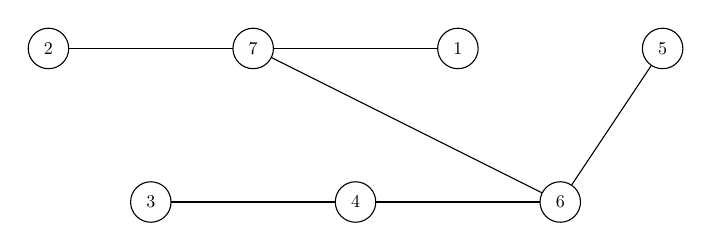
\begin{tikzpicture}[vertex/.style = {shape=circle,draw,minimum size=2.25em},scale=0.65, every node/.style={scale=0.65}]
    \node[vertex] (c1) at (0,3) {$1$};
    \node[vertex] (c2) at (-8,3) {$2$};
    \node[vertex] (c3) at (-6,0) {$3$};
    \node[vertex] (c4) at (-2,0) {$4$};
    \node[vertex] (c5) at (4,3) {$5$};
    \node[vertex] (c6) at (2,0) {$6$};
    \node[vertex] (c7) at (-4,3) {$7$};
    \draw (c6) -- (c7);
    \draw (c5) -- (c6);
    \draw (c4) -- (c6);
    \draw (c3) -- (c4);
    \draw (c2) -- (c7);
    \draw (c1) -- (c7);
\end{tikzpicture}